\documentclass{article}

\author{Джоуни Суннари}
\title{Курсовик}
\usepackage[utf8]{inputenc}
\usepackage[russian]{babel}
\usepackage{graphicx}
\usepackage{listings}
\usepackage{color}
\usepackage{cite}

\begin{document}
\maketitle
\pagebreak
\tableofcontents
\pagebreak

\newcommand{\myparagraph}[1]{\paragraph{#1}\mbox{}\\}

\section{Теоритический этап}
% определение понятий «информационная система»,
% используемых видов архитектур ИС, элементов, составляющих используемые виды
% архитектур, других специальных понятий, используемых в курсовой работе;

\pagebreak

\section{Анализ и моделирование процессов}
% сбор, анализ и
% систематизация информации об объекте автоматизации в рамках выбранной тематики КР,
% моделирование деятельности предприятия, отдельного контура управления предприятием,
% процессов, автоматизируемых выбранным программным средством (средствами),
% формирование требований к средствам автоматизации

% Все процессы можно не брать
% Процессы - это как в первой лабе
% близко рассматривать можно только одну систему

\subsection{Описание прикладных и бизнес-процессов}
%   В рамках тематики 2 предполагается описание деятельности предприятия в целом,
% места в его деятельности выбранного контура управления, процессов, реализуемых в этом
% контуре и связанных с ними информационных процессов (какие процессы сбора,
% обработки, хранения, передачи и предоставления информации реализованы в этом
% контуре и насколько они формализованы), информационных объектов, которые
% используются в этих процессах (планы, графики, спецификации, договора, наряды,
% реестры и т.п.).

Компания занимается продажей билетов за организаторов мероприяий.


\subsubsection{описание деятельности предприятия в целом}
Продажа билетов происходит на сайте компании, через виджеты на сайте, в соцсетях организатора,
через билетных операторов Яндекс.Афиша, Kassir.ru, Muzbilet, Parter.ru и других.
Предостовляет оборудование и ПО для продажи билетов в кассе
и организации контроля управления доступом (печать и сканарование билетов).

В личном кабинете организатора есть возможность создания событий,
смотреть статистику о продажах и скачивать отчёты, так же есть
инструменты для работы с ценами и повышения лояльности зрителей (абонементы, промокоды).
Также есть функционал по началу рекламных кампаний и рассылке.

Есть централизованная служба поддержки покупателей (возвраты, консультации) \cite{radario}.

\paragraph{выделяеться несколько контуров управления}
\begin{enumerate}
    \item{работа с организаторами, заключение договоров и т.д.}
    \item{работа с клиентами организаторов}
    \item{техподдержка организаторов, помощь в ПО}
    \item{маркетинг}
    \item{разработка, тестирование}
    \item{найм сотрудников}
\end{enumerate}

\subsubsection{место разработки в деятельности предприятия}

Разработка занимает важное место в деятельности компании.
Так как основным продуктом компании является упрощение продаж билетов и контроль
за ними, а всё это реализовано, через личный кабинет на сайте, нужно всё это разрабатывать
и поддерживать.

\paragraph{Процессы контура управления разработка \cite{wiki}}
\begin{enumerate}
    \item{распределение задач на спринт}
    \item{выполнение задачи}
    \item{проверка кода другим человеком}
    \item{тестирование}
    \item{развертывание}
\end{enumerate}

После распределения задач у каждого разработчика есть назначенные на него задачи с описанием.
Во время выполнения задачи по мимо написания кода разработчик меняет статус задачи,
создаёт подзачачи, если они понадобятся для выполнения основной задачи.
Перед проверкой кода другим человеком, разработчик состовляет подробное техническое описание
вошедших изменений. Затем он назначает другого разработчика на проверку,
меняет статус задачи, и если это новый сервис то пишет статью о нём во внутренний справочник.
Так же добовляет во внутренний справочник все изменения,
которые в последствии рассылаются по корпоративной почте.
При просмотре изменений человек либо пишет замечания и отправляет на доработку,
либо одобряет изменения. В последнем случае разработчик отправлявший свой код на проверку
отправляет его на тесты, изменив статус задачи. Тестировщик когда-нибудь проверит эту задачу,
и изменит ей статус, тогда разработчик начнет развертывать код на серверах.
Он будет делать это либо вручную (если это микросервис), 
либо автоматически (если автоматическая сборка и автотесты уже настроены).
На время развёртывания основных проектов (не микросервисов) другим разработчикам нужно подождать
чтобы не развёртывать одновременно. Для этой цели о развёртываниях пишутся сообщения в чат в slack.
\cite{wiki}

\paragraph{информационные объекты}
\begin{enumerate}
    \item{описание задачи}
    \item{опиасние к коду}
    \item{сообщения в корпоративной почте}
    \item{сообщения в slack о развертываниях}
    \item{статьи во внутреннем справочнике}
\end{enumerate}


\pagebreak


\subsection{Формализованное визуальное моделирование и формирование требований}
% Выбирается методология и в соответствии с ее правилами формируется набор
% диаграмм, дающих формальное описание процессов. Модели должны демонстрировать
% анализируемые процессы с точностью до отдельных операций, позволять для этих
% операций определить акторов и информационные объекты, использующиеся в них.
% Делаются выводы о функциональных требованиях к средствам автоматизации со стороны
% смоделированных процессов. Для второй тематики обязательно, а для первой и третьей
% тематики рекомендуется описать нефункциональные требования (к производительности,
% надежности, безопасности и т.п.) к средствам автоматизации и обосновать их исходя из
% приведенных выше описаний и моделей.

\newcommand{\dia}[2]{
    \begin{figure}[!h]
        \includegraphics[width=\textwidth]{#1}
        \caption{#2 \cite{wiki}}
    \end{figure}
    \pagebreak
}

\begin{figure}[h!]
    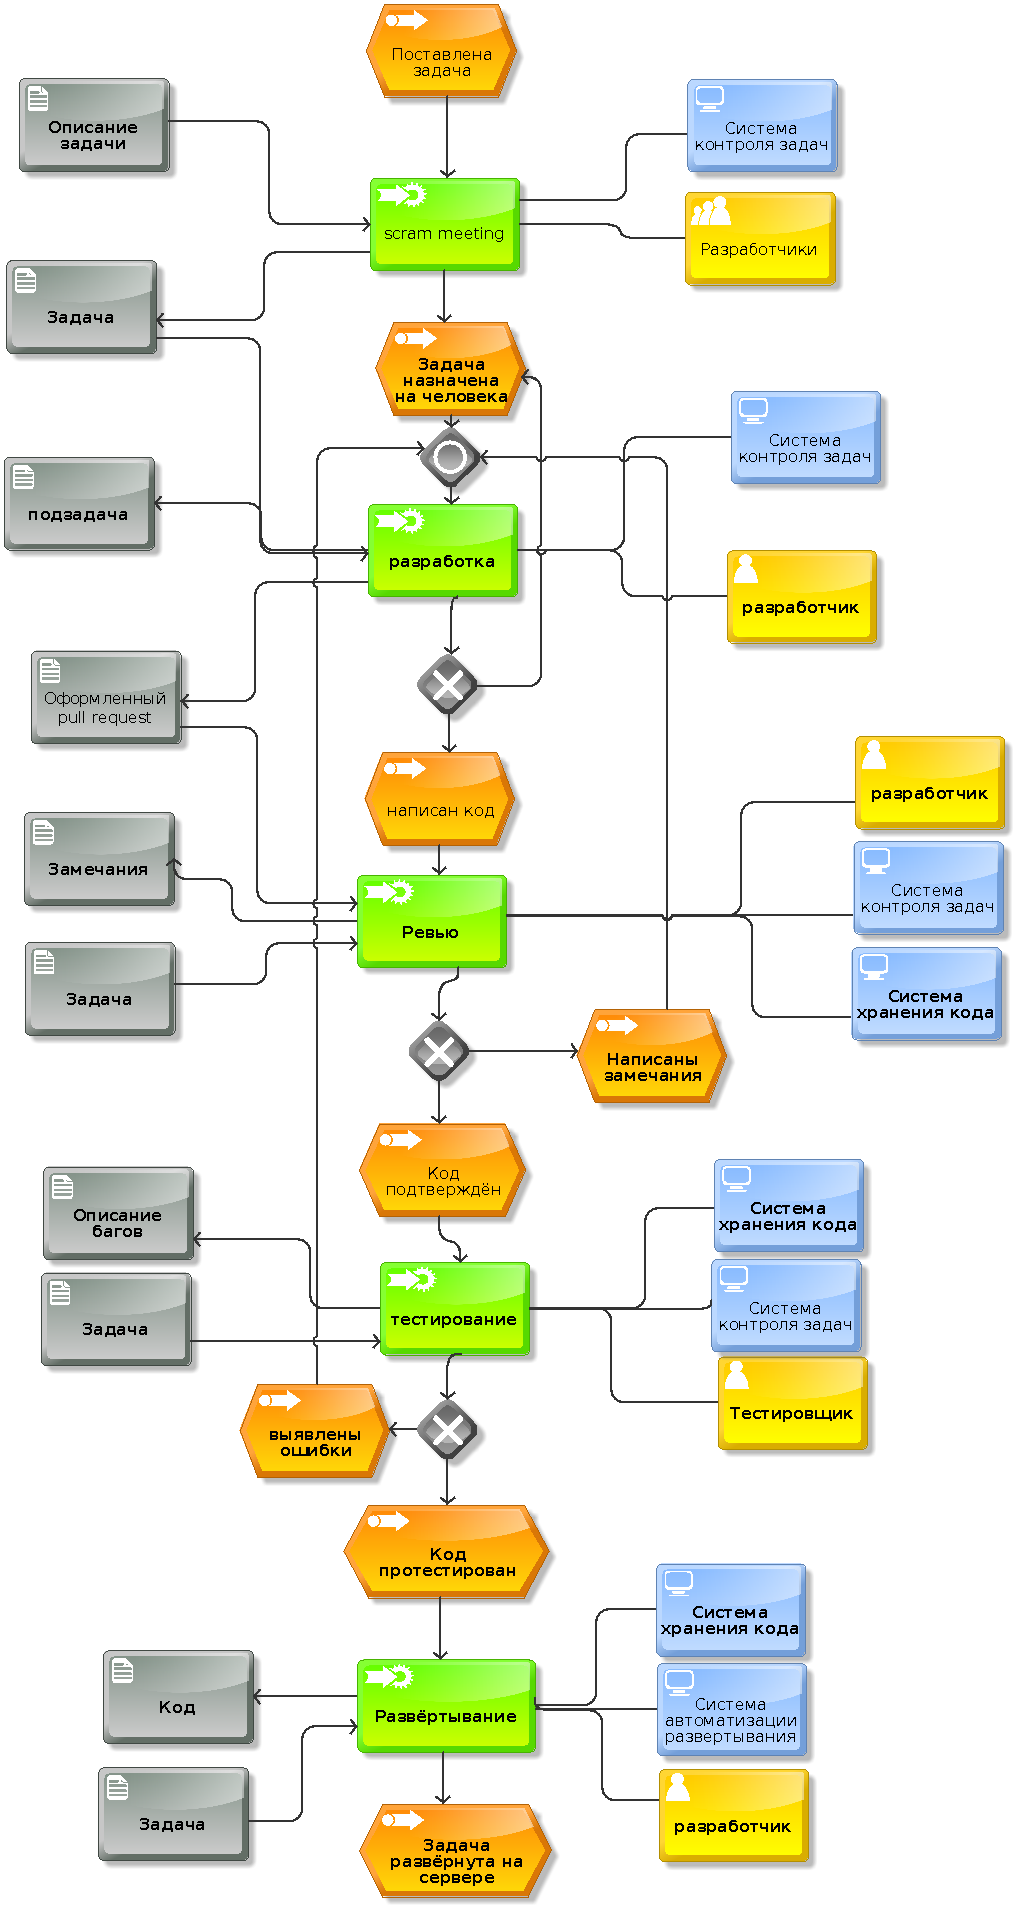
\includegraphics[height=6in]{pictures/2.png}
    \caption{контур разработки \cite{wiki}}
\end{figure}
\pagebreak
\dia{pictures/3.png}{scram meeting}
\dia{pictures/4.png}{разработка}
\dia{pictures/5.png}{ревью}
\dia{pictures/7.png}{развёртывание}

\subsection{функциональные требования}
\paragraph{Система слежения за задачами}
\begin{enumerate}
    \item{у задачи должны быть множество статусов:
    открыта, в процессе, готова к ревью, готова к тестированию, готова к развёртыванию, работа завершена}
    \item{должно быть видно кто работает над задачей, кто её тестирует, а также её описание}
    \item{должна быть возможность добавлять подзадачи}
    \item{возможность оценивания времени, требуемого для решения}
    \item{возможность создавать задачи, назначать их на людей, распределять по приоритету}
    \item{нужно чтобы у системы было API}
    \item{нужна интеграция с системой хранения кода}
\end{enumerate}

\paragraph{Системе хранения кода}
\begin{enumerate}
    \item{возможность удобно смотреть разницу в коде}
    \item{оставление комментариев, замечаний}
    \item{запрет на слияние без ревью}
    \item{составление описания изменения}
    \item{нужно чтобы у системы было API}
\end{enumerate}

\paragraph{Система автоматического развертывания}
\begin{enumerate}
    \item{гибкие настройки связи с сервером развёртывания}
    \item{интеграция с системой хранения кода}
    \item{возможность запуски автотестов перед развёртыванием}
    \item{мониторинг за процессом, просмотр ошибок компиляции}
    \item{нужно чтобы у системы было API}
\end{enumerate}

\subsection{нефункциональные требования}
\paragraph{Система хранения кода}
\begin{enumerate}
    \item{код не должен попасть в чужие руки}
    \item{возможность настройки прав для доступа к репохиториям и слияния с основной веткой}
    \item{безопастность и надежность сдесь важнее производительности (лучше подождать немного, чем в один прекрасный момент потерять весь свой код, или обнаружить что кто-то другой получил доступ к нему).}
\end{enumerate}

\paragraph{Cистема контроля задач}
\begin{enumerate}
    \item{не накладываются большие требования по безопасности (в пользу удобства работы, надежности и производительности)}
    \item{она должна быть производительна, т.к. не продполагается выделение производительных серверов под эту систему.}
    \item{надежность тоже требуется высокая чтобы работа не останавливалась.}
\end{enumerate}

\paragraph{Cистема развертывания}
\begin{enumerate}  
    \item{должна быть система прав}
   
    \item{в этой системе предполагается долтуп к серверам, на которых будет происходить развёртывание.
    поэтому она должна быть безопасная, чтобы никто не смог получить к ней доступ, или используя уязвимость
    получить доступ к серверам.}
   
    \item{компиляция - требовательная по ресурсам операция. Нужно что бы она не мешала обрабатывать серверам запросы.
    должна быть возможность производить сборку на отдельных серверах, чтобы не перегружать существующие.}
   
    \item{система должна быть надёжна, так как если она сломается, никто не будет знать что делать, так как все привыкнут
    её использовать и не будут знать как происходит механизм развертывания.}
\end{enumerate}   

\pagebreak


\section{Анализ средств автоматизации процессов}
% сбор, анализ и
% систематизация информации о средствах автоматизации в рамках выбранной тематики
% КР: функциональных возможностях, реализуемых информационных объектах,
% требованиях к инфраструктуре и способах развертывания, программных компонентах и
% способах их взаимодействия, структурах данных и организации хранилищ данных и т.п.

%   В рамках тематики 2 предполагается структурированное описание
% функциональных возможностей одного или нескольких средств автоматизации,
% применяющихся для автоматизации определенных на предыдущем этапе процессов,
% обоснование возможности их применения (рекомендуется также обосновать выбор
% конкретных средств), сопоставление их функциональных возможностей с требованиями
% процессов, детальное описание требований к ИТ-инфраструктуре со стороны выбранных
% программных средств, рекомендуемых производителем вариантов развертывания этих
% средств и средств их интеграции между собой и с внешними системами.

Для автоматизации выше описанных процессов в предприятии применяются github.com как система хранения кода,
YouTrack, как система отслеживания задач и управления проектом, и TeamCity, как система автоматического развёртывания.

\myparagraph{github.com}

Эта система соответствует всем функциональным требованиям.\\
Она не может быть развёрнута на своих серверах, распространяется как SaaS решение.
Это может быть для кого-то неудобством, но для предприятия, исследуемого в данной курсовой работе, неудобством это не является.
Наоборот удобнее использовать SaaS решение, чем самим арендовать сервера и развёртывать там, и потом следить за ним, что повлечёт дополнительные расходы.

Тут может возникнуть вопрос по поводу надежности и безопастности: "Может не стоит доверять свой код какой-то огранизации?". Однако это не хуже
чем доверять код своим сотрудникам. Они могут совершить ошибку с гораздо большей вероятностью, чем администраторы системы, так как администрирование
системы хранения кода - не основная их задача.

Интегрировать систему с другими лучше всего с помощью клиентов уже написанных клиентов https://github.com/octokit, а если на нужном языке программирования его нет,
придется написать своего, использующего API.
\\\\
\textbf{функциональные возможности}
\begin{enumerate}
    \item{возможность создавать команды для ограничения прав}
    \item{ограничение слияния с основной веткой}
    \item{удобный просмотр разницы в коде}
    \item{есть API, клиенты для .NET, Go, JavaScript}
\end{enumerate}


\myparagraph{YouTrack}

Система с избытком отвечает функциональным требованиям.\\
Развернуть можно на своём сервере (в докере или jar) или на серверах jetbrains.
При развертывании на своих серверах потребуется core i3, 1GB disk, 1.5 Gb RAM. \cite{youtrack_requirements}
Однако удобнее развернуть на сервере jetbrains (потому же почему и github).

Интеграция с другими системами (guthub.com) есть встроенная, однако если её не достаточно, воспользоватся клиентом на .NET
YouTrackSharp, или же неписать своего, использующего доступный API.
\\\\
\textbf{функциональные возможности \cite{youtrack}}
\begin{enumerate}
    % Connect external tools with YouTrack to enhance your productivity and improve your working process! Integrate with TeamCity to automatically set the value for the ‘Fixed in build’ field in YouTrack when an issue is closed in a successful build.
    \item{интеграция с GitHub, Bitbucket, GitLab для доступа к коммитам. Интеграция с TeamCity.}
    %YouTrack lets you track and manage issues from the moment they’re reported to the moment they’re fixed. Easily create issues, add tags, watchers, modify custom fields, set the priority, and edit added attachments with a built-in image editor. Configure your personal notifications.
    \item{слежение и управление задачами(issue) момента создания до момента выполнения. Создание задач, добавление тэгов, изменение пользовательских полей, установление приоритета, настройка уведомлений}
    % Agile boards in YouTrack are designed to help teams follow a wide range of agile project management processes. You can create Scrum, Kanban, or Scrumban boards.
    \item{Agile доски}
    % A variety of reports are available to help you analyze and manage projects and teams activities. Create private reports or configure reports that you share with your team.
    \item{различные отчёты для анализирования и управления проектами}
    
    % The Time Tracking features let you and your team report the amount of time spent working on issues in your project. Estimate how much time you expect to spend to resolve each issue, add work items to the issues along with the spent time, and create summary reports to see the total amount of time spent on the different types of work.
    \item{слежение за временем}
    % YouTrack is very customizable! Whether it’s issue fields, workflows, notifications or a language – you can configure it all to your needs.
    \item{добавление пользовательских полей к задачам и Agile доскам}
    \item{есть API, клиенты для .NET и PHP}
\end{enumerate}

\myparagraph{TeamCity}

Система отвечает функциональным требованиям.
Сам TeamCity состоит из http сервера и нескольких build agent'ов.
Для одного из них потребуется 2GB RAM, dual-core CPU, 10GB долговременной памяти \cite{octopus}.
Агентов лучше размещать на отдельных серверах, чтобы не перегружать первые, так как сборка - ресурсоёмкая и длительная по времени операция.

Интеграция с системами контроля версий доступны "из коробки", также при желании можно воспользоватся API, или, что гораздо удобнее,
готовым клиентом на kotlin https://github.com/JetBrains/teamcity-rest-client
\\\\
\textbf{функциональные возможности \cite{teamcity}}
\begin{enumerate}
    \item{интеграция c CVS}
    % Build, check and run automated tests on the server even before committing your changes – keeping your code base clean at all times.
    \item{сборка и запуск автотестов перед коммитом изменений}
    % Form your project tree to inherit parent settings and permissions.
    % Templates
    \item{иерархия проектов в виде дерева для наследования настроек и прав}
    % Create templates with common settings and inherit any number of build configurations from them.
    \item{создание шаблонов}
    % Build chains and dependencies
    \item{создание зависимостей}
    % Break down a single build procedure into parts that can be run in sequence or in parallel.
    \item{разбитие процедуры на части для возможности запуска  параллельно}
    \item{есть отдельно сервер TeamCity и множество build agent'ов}
    \item{есть API и клиент на kotlin}
\end{enumerate}
\pagebreak

\section{Синтез определенных уровней архитектуры ИС}
% (непосредственно проектирование архитектуры ИС на уровне (уровнях), определяемых
% тематикой КР: функциональной архитектуры, информационной архитектуры, системнойархитектуры, программной архитектуры, архитектуры данных, обоснование соответствия
% построенной архитектуры требованиям процессов).

%   В рамках тематики 2 предполагается построение системной архитектуры.
% Необходимо обосновать выбор способа развертывания определенного на предыдущем
% этапе средства автоматизации (или нескольких), включая обоснование количество и
% размещение серверных компонентов, в том числе с использованием технологий
% виртуализации, выбор телекоммуникационных технологий, операционных систем,
% базового программного обеспечения. В описание полученной системной архитектуры
% включаются аппаратные узлы для размещения как серверных, так и клиентских
% компонентов системы, периферийное оборудование, телекоммуникационное
% оборудование, любое системное или вспомогательное программное обеспечение.
% Обосновывается соответствие построенной архитектуры функциональным и
% нефункциональным требованиям, определенным на первом этапе и требованиям к ИТ-
% инфраструктуре со стороны программных средств автоматизации, указанным на втором
% этапе. Указывается за счет каких архитектурных решений обеспечивается требуемый
% уровень производительности (в том числе в условиях изменяющейся нагрузки),
% надежности и безопасности ИС. Описание спроектированной архитектуры
% сопровождается диаграммами, выполненными в соответствии с требованиями нотации
% UML.

\newcommand{\diaa}[2]{
    \begin{figure}[!h]
        \includegraphics[width=\textwidth]{#1}
        \caption{#2}
    \end{figure}
}
Реализована асинхронная балансировка нагрузки c 2мя балансировщиками (если один упадёт, другой на подхвате). Так же есть 2 сервера с базами данных 4 пары файл серверов.
\diaa{diags/1.png}{Архитектура github.com \cite{github}}

The first thing your request hits after coming down from the internet is the active load balancer. For this task we use a pair of Xen instances running ldirectord. These are called lb1a and lb1b. At any given time one of these is active and the other is waiting to take over in case of a failure in the master. The load balancer doesn’t do anything fancy. It forwards TCP packets to various servers based on the requested IP and port and can remove misbehaving servers from the balance pool if necessary. In the event that no servers are available for a given pool it can serve a simple static site instead of refusing connections.
\diaa{diags/2.png}{балансировщик \cite{github,nmap_github}}
\pagebreak

Many pages require database lookups. Our MySQL database runs on two 8 core, 32GB RAM bare metal servers with 15k RPM SAS drives. Their names are db1a and db1b. At any given time, one of them is master and one is slave. MySQL replication is accomplished via DRBD.
\diaa{diags/databases.png}{базы данных \cite{github}}

Once the Smoke proxy has determined the user’s route, it establishes a transparent proxy to the proper file server. We have four pairs of fileservers. Their names are fs1a, fs1b, …, fs4a, fs4b. These are 8 core, 16GB RAM bare metal servers, each with six 300GB 15K RPM SAS drives arranged in RAID 10. At any given time one server in each pair is active and the other is waiting to take over should there be a fatal failure in the master. All repository data is constantly replicated from the master to the slave via DRBD.

The above flow is what happens when there are no cache hits. In many cases the Rails code uses Evan Weaver’s Ruby memcached client to query the Memcache servers that run on each slave file server. Since these machines are otherwise idle, we place 12GB of Memcache on each. These servers are aliased as memcache1, …, memcache4.
\diaa{diags/file-server.png}{файл сервера \cite{github}}
\pagebreak

For requests to the main website, the load balancer ships your request off to one of the four frontend machines. Each of these is an 8 core, 16GB RAM bare metal server. Their names are fe1, …, fe4. Nginx accepts the connection and sends it to a Unix domain socket upon which sixteen Unicorn worker processes are selecting. One of these workers grabs the request and runs the Rails code necessary to fulfill it.
\diaa{diags/frontend.png}{frontend сервер \cite{github}}
\pagebreak

First, your Git client initiates an SSH session. The connection comes down off the internet and hits our load balancer.

From there, the connection is sent to one of the frontends where SSHD accepts it. We have patched our SSH daemon to perform public key lookups from our MySQL database. Your key identifies your GitHub user and this information is sent along with the original command and arguments to our proprietary script called Gerve (Git sERVE). Think of Gerve as a super smart version of git-shell.

Gerve verifies that your user has access to the repository specified in the arguments. If you are the owner of the repository, no database lookups need to be performed, otherwise several SQL queries are made to determine permissions.

Once access has been verified, Gerve uses Chimney to look up the route for the owner of the repository. The goal now is to execute your original command on the proper file server and hook your local machine up to that process. What better way to do this than with another remote SSH execution!

I know it sounds crazy but it works great. Gerve simply uses exec(3) to replace itself with a call tossh git@<route> <command> <arg>. After this call, your client is hooked up to a process on a frontend machine which is, in turn, hooked up to a process on a file server.

Think of it this way: after determining permissions and the location of the repository, the frontend becomes a transparent proxy for the rest of the session. The only drawback to this approach is that the internal SSH is unnecessarily encumbered by the overhead of encryption/decryption when none is strictly required. It’s possible we may replace this this internal SSH call with something more efficient, but this approach is just too damn simple (and still very fast) to make me worry about it very much.

Tracing a Git Request

Performing public clones and pulls via Git is similar to how the SSH method works. Instead of using SSH for authentication and encryption, however, it relies on a server side Git Daemon. This daemon accepts connections, verifies the command to be run, and then uses fork(2) and exec(3) to spawn a worker that then becomes the command process.

With this in mind, I’ll show you how a public clone operation works.

First, your Git client issues a request containing the command and repository name you wish to clone. This request enters our system on the load balancer.

From there, the request is sent to one of the frontends. Each frontend runs four ProxyMachine instances behind HAProxy that act as routing proxies for the Git protocol. The proxy inspects the request and extracts the username (or gist name) of the repo. It then uses Chimney to lookup the route. If there is no route or any other error is encountered, the proxy speaks the Git protocol and sends back an appropriate messages to the client. Once the route is known, the repo name (e.g. mojombo/bert) is translated into its path on disk (e.g. a/a8/e2/95/mojombo/bert.git). On our old setup that had no proxies, we had to use a modified daemon that could convert the user/repo into the correct filepath. By doing this step in the proxy, we can now use an unmodified daemon, allowing for a much easier upgrade path.

Next, the Git proxy establishes a transparent proxy with the proper file server and sends the modified request (with the converted repository path). Each file server runs two Git Daemon processes behind HAProxy. The daemon speaks the pack file protocol and streams data back through the Git proxy and directly to your Git client.

Once your client has all the data, you’ve cloned the repository and can get to work!
\diaa{diags/github.png}{часть архитектуры \cite{github,nmap_github}}
\pagebreak

Компания использует YouTrack, и github.com как облачные сервисы, а TeamCity развертывает на арендованном сервере. Как видно из диаграммы, и агент сборки и сервер, предоставляющий web интерфейс, развёрнуты на одном отдельном сервере. Таким образом нет дополнительной нагрузки на основные сервера во время сборки.
Одного агента сборки хватает, поэтому нет смысла пока изменять архитектуру.
\diaa{diags/Diagram1.png}{Часть архитектуры предприятия \cite{nmap_build_server,nmap_prod_server,nmap_youtrack_server}}
\pagebreak

\pagebreak

\section{Список использованных источников}

\begin{thebibliography}{9}
    \bibitem{github}  
    \textit{blog.github.com/2009-10-20-how-we-made-github-fast/}
     
    \bibitem{xen}
    \textit{wiki.xenproject.org/wiki/Xen\_Project\_Beginners\_Guide}
     
    \bibitem{radario}
    \textit{business.radario.ru}

    \bibitem{wiki}
    \textit{приватная вики на гитхабе}

    \bibitem{youtrack}
    \textit{jetbrains.com/youtrack/features/}

    \bibitem{youtrack_requirements}
    \textit{youtrack-support.jetbrains.com/hc/en-us/articles/206546119-What-hardware-requirements-does-YouTrack-have-}

    \bibitem{octopus}
    \textit{octopus.com/docs/installation/requirements}

    \bibitem{teamcity}
    \textit{jetbrains.com/teamcity/features/}

результаты сканирования серверов

\bibitem{nmap_github}
\begin{lstlisting}[language=bash, basicstyle=\ttfamily\small]
    $ nmap -O github.com
\end{lstlisting}
\begin{lstlisting}[frame=lines, basicstyle=\ttfamily\small]
    ...
    PORT     STATE SERVICE
    22/tcp   open  ssh
    80/tcp   open  http
    443/tcp  open  https
    9418/tcp open  git
    Warning: OSScan results may be unreliable because we could not find at least 1 open and 1 closed port
    Device type: specialized|storage-misc
    Running (JUST GUESSING): Crestron 2-Series (87%), HP embedded (85%)
    OS CPE: cpe:/o:crestron:2_series cpe:/h:hp:p2000_g3
    Aggressive OS guesses: Crestron XPanel control system (87%), HP P2000 G3 NAS device (85%)
    No exact OS matches for host (test conditions non-ideal).
\end{lstlisting}

\bibitem{nmap_youtrack_server}
\begin{lstlisting}[language=bash, basicstyle=\ttfamily\small]
    $ nmap -O ***.myjetbrains.com
\end{lstlisting}
\begin{lstlisting}[frame=lines, basicstyle=\ttfamily\small]
    ...
    PORT    STATE SERVICE
    80/tcp  open  http
    443/tcp open  https
    Warning: OSScan results may be unreliable because we could not find at least 1 open and 1 closed port
    Device type: general purpose|phone|WAP|PBX
    Running (JUST GUESSING): Linux 3.X|4.X|2.6.X (97%), Google Android 4.X|4.1.X (91%), Vodavi embedded (87%)
    OS CPE: cpe:/o:linux:linux_kernel:3 cpe:/o:linux:linux_kernel:4 cpe:/o:google:android:4.0 cpe:/o:google:android:4.1.2 cpe:/o:linux:linux_kernel:3.18 cpe:/o:linux:linux_kernel:4.1 cpe:/o:linux:linux_kernel:2.6.32 cpe:/h:vodavi:xts-ip
    Aggressive OS guesses: Linux 3.10 - 4.11 (97%), Android 4.0 (91%), Android 4.1.2 (90%), OpenWrt Chaos Calmer 15.05 (Linux 3.18) or Designated Driver (Linux 4.1 or 4.4) (90%), DD-WRT v3.0 (Linux 4.4.2) (90%), Linux 2.6.32 (90%), Linux 3.2 - 3.10 (90%), Linux 3.2 - 3.16 (90%), Linux 3.2 - 3.8 (90%), Linux 3.18 (89%)
    No exact OS matches for host (test conditions non-ideal).
    ...
\end{lstlisting}

\bibitem{nmap_prod_server}
\begin{lstlisting}[language=bash, basicstyle=\ttfamily\small]
    $ nmap -O m***.ru
\end{lstlisting}
\begin{lstlisting}[frame=lines, basicstyle=\ttfamily\small]
    ...
    PORT    STATE SERVICE
    80/tcp  open  http
    443/tcp open  https
    Warning: OSScan results may be unreliable because we could not find at least 1 open and 1 closed port
    Device type: general purpose
    Running: Microsoft Windows 2012
    ...
\end{lstlisting}
\bibitem{nmap_build_server}
\begin{lstlisting}[language=bash, basicstyle=\ttfamily\small]
    $ nmap -O -Pn bo**.ru
\end{lstlisting}
\begin{lstlisting}[frame=lines, basicstyle=\ttfamily\small]
    ...
    PORT     STATE SERVICE
    80/tcp   open  http
    81/tcp   open  hosts2-ns
    3389/tcp open  ms-wbt-server
    9090/tcp open  zeus-admin
    Warning: OSScan results may be unreliable because we could not find at least 1 open and 1 closed port
    Device type: general purpose|phone
    Running (JUST GUESSING): Microsoft Windows 2012|10|7|Phone (92%), FreeBSD 6.X (85%)
    ...
\end{lstlisting}
\end{thebibliography}

\end{document}
